\documentclass[preview]{standalone}

\usepackage{amsmath}
\usepackage{amssymb}
\usepackage{stellar}
\usepackage{definitions}
\usepackage{tikz}
\usepackage{boldline}
\usepackage{amsthm}
\usepackage{makecell}

\begin{document}

\id{geometric-groups}
\genpage

\section{Introduction}

\begin{snippetdefinition}{isometry-definition}{Isometry}
    Let \((\pi, d)\) be a \metricspace.
    A \function
    \[
        \sigma\colon \pi \cartesianprod \pi \fromto \realnumbers
    \]
    is an \textit{isometry} if
    \[
        \forall P, Q \in P, d(P, Q) = d(\sigma(P), \sigma(Q))
    \]
\end{snippetdefinition}

\begin{snippetproposition}{isometry-is-bijective}{Isometry is bijective}
    An \isometry is \bijective.
\end{snippetproposition}

\begin{snippetproposition}{isometry-sends-lines-to-lines}{}
    An \isometry sends every line to a line.
\end{snippetproposition}

% Questo si dimostra con la disuglianza triangolare notando che il segno uguale
% vale solo quando un punto si trova sulla retta fra gli altri due punti.

\begin{snippetproposition}{isometry-tre-points}{Isometry 3 points}
    Let \(\sigma\) and \(\tau\) be \isometry[isometries].
    If the \isometry[isometries] coincide on \(3\) unaligned
    points, then \(\sigma = \tau\).
\end{snippetproposition}

\begin{snippettheorem}{isometries-subgroup-theorem}{Isometries as symmetric group}
    The \isometry[isometries] of a plane \(\pi\)
    are a \subgroup of \(\symgrp(\pi)\).
\end{snippettheorem}

\begin{snippetproof}{isometries-subgroup-theorem-proof}{isometries-subgroup-theorem}{Isometries as symmetric group}
    The subset of \isometry[isometries] contains the identity element
    of \(\symgrp(\pi)\), which is the identity function.
    If \(\sigma\) and \(\tau\) are \isometry[isometries], then
    \(\tau(\sigma)\) is an \isometry. Given \(P, Q \in \pi\)
    we have
    \[
        d(P, Q) = d(\sigma(P), \sigma(Q)) = d(\tau(\sigma(P)), \tau(\sigma(Q)))
    \]
    If \(\sigma\) is an \isometry, we know that it is invertible.
    We now show that \(\sigma^\inversefunction\) is an \isometry.
    Given \(P, Q \in \pi\), consider 
    \[
        d(\sigma^\inversefunction(P), \sigma^\inversefunction(Q))
        = d(\sigma^\inversefunction(\sigma^\inversefunction(P)), \sigma^\inversefunction(\sigma^\inversefunction(Q)))
        = d(P, Q)
    \]
\end{snippetproof}

\plain{The set of translations form a subgroup of the isometries, but the rotations
do not. Only the rottions with the same center do.}

\plain{Given two lines with a common point, any isometry will keep the point still,
resulting in a rotation centered on the intersection of the two lines.}

\begin{snippetproposition}{preserving-isometries-subgroup}{Preserving isometry}
    Let \(F\subseteq \pi\). Consider the \isometry[isometries]
    \(\sigma\) such that \(\sigma(F) = F\).
    Then, these \isometry[isometries] form a \subgroup of \(\symgrp(\pi)\).
\end{snippetproposition}

\plain{Note: this does not mean that every point is preserved. Consider, for instance,
a rotation of a circle with respect to its center, or a 90 degree rotation of a square
with respect to its center.}

\section{Dihedral group}

\begin{snippetdefinition}{dihedral-group-definition}{Dihedral group}
    Consider a regular polygon with \(n > 2\) sides.
    The \textit{dihedral group} is the \group
    of \isometry[isometries] that send the polygon to itself.
    \[
        D_{2n}
    \]
\end{snippetdefinition}

\plain{Such isometries send sides to side and vertices to vertices.}

\begin{snippet}{nth-polygon-illustration}
    \begin{center}
        \begin{tikzpicture}
            \newdimen\R
            \R=2cm
    
            \draw (-40:\R)
    
            \foreach [count=\n] \x in {0,40,...,240} {
                -- (\x:\R) node [anchor=180+\x] {\n}
            };
    
            \draw (-40:\R) node [anchor=140] {$n$};
            \draw[dashed] (240:\R) arc [start angle=240, end angle=320, radius=\R];
    
          \end{tikzpicture}
    \end{center}
\end{snippet}

\plain{Note that three vertices suffice to reconstruct the entire isometry.}

\begin{snippettheorem}{dihedral-group-order-theorem}{Dihedral group order}
    Let \(n > 2\). Then,
    \[
        |\dihedralgrp_{2n}| = 2n
    \]
\end{snippettheorem}

\begin{snippetproof}{dihedral-group-order-theorem-proof}{dihedral-group-order-theorem}{Dihedral group order}
    Consider the vertices labelled \(n, 1, 2\).
    We can choose the image of \(1\)
    in \(n\) ways. Once an image of \(1\) is chosen, the vertices
    \(n\) the vertices \(n\) and \(2\)
    need to go to the adjacent vertices of the image.
    We have at most two possibilities. Thus, we have \(2n\) possible combinations.
\end{snippetproof}

\begin{snippetproposition}{dihedral-group-not-abelian}{Dihedral group not abelian}
    Let \(n > 2\). Then, \(\dihedralgrp_{2n}\) is not an \abeliangroup.
\end{snippetproposition}

\begin{snippetproof}{dihedral-group-not-abelian-proof}{dihedral-group-not-abelian}{Dihedral group not abelian}
    Consider the rotation \(\rho\) which sends the vertex \(1\) into \(2\), so
    every vertex is sent into the next vertex and \(n\) is sent to \(1\),
    and the symmetry \(\sigma\) which fixes vertex \(1\).
    If we apply \(\rho\) and then \(\sigma\), the vertex \(1\) is sent to \(n\).
    If we apply \(\sigma\) and then \(\rho\), the vertex is sent to \(2\).
\end{snippetproof}

\section{T-group or Klein group}

\begin{snippet}{rectangle-label-illustration}
    \begin{center}
        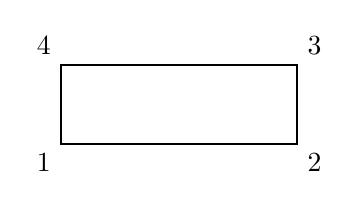
\begin{tikzpicture}
            % Draw a rectangle and label vertices
            \draw[thick] (0,0) node[below left] {1} 
                         -- (3,0) node[below right] {2}
                         -- (3,1) node[above right] {3}
                         -- (0,1) node[above left] {4} 
                         -- cycle;
        \end{tikzpicture}
    \end{center}
\end{snippet}

\begin{snippet}{klein-group-expl}
    Consider an \isometry that sends a non-square rectangle to itself.
    This function must send vertices to vertices. The possible images for the first
    vertices are \(4\). Once the first vertex is fixex, the others follow
    (the smaller sides to to the smaller sides and such). Thus, there are  \(4\)
    elements in this group:
    \begin{enumerate}
        \item the identity;
        \item two axial symmetries;
        \item central symmetry.
    \end{enumerate}
\end{snippet}

\begin{snippet}{klein-group-cayley}
    Let \(\rho\) and \(\sigma\) be the axial symmetries and \(\tau\)
    the central symmetry.
    \begin{center}
        \bgroup{}
        \def\arraystretch{1.25}
        \begin{tabular}{|c !{\vrule width0.8pt} c|c|c|c|}
            \hline
            \phantom{ } & \(\identityfunc\) & \(\sigma\) & \(\rho\) & \(\tau\) \\
            \Xhline{0.8pt}
            \(\identityfunc\) & \(\identityfunc\) & \(\sigma\) & \(\rho\) & \(\tau\) \\
            \hline
            \(\sigma\) & \(\sigma\) & \(\identityfunc\) & \(\tau\) & \(\sigma\) \\
            \hline
            \(\rho\) & \(\rho\) & \(\tau\) & \(\identityfunc\) & \(\sigma\) \\
            \hline
            \(\tau\) & \(\tau\) & \(\rho\) & \(\sigma\) & \(\identityfunc\) \\
            \hline
        \end{tabular}
        \egroup{}
    \end{center}
    \phantom{}
\end{snippet}

\plain{The Cayley table of the Klein group is the table of a group of order four.
}

\end{document}